\documentclass{article}

% Language setting
% Replace `english' with e.g. `spanish' to change the document language
\usepackage[english]{babel}

% Set page size and margins
% Replace `letterpaper' with`a4paper' for UK/EU standard size
\usepackage[letterpaper,top=2cm,bottom=2cm,left=3cm,right=3cm,marginparwidth=1.75cm]{geometry}

% Useful packages
\usepackage{amsmath}
\usepackage{graphicx}
\usepackage[colorlinks=true, allcolors=blue]{hyperref}

\title{\textbf{Assessment\\CASA0002 Urban Simulation\\MSc Urban Spatial Science}}
\author{\textbf{Andrés Restrepo Jiménez}}

\usepackage{natbib}
\bibliographystyle{abbrvnat}
\hypersetup{citecolor=black}
\setcitestyle{authoryear,open={(},close={)}}
\setcounter{secnumdepth}{4}

\begin{document}
\maketitle

% \begin{abstract}
% Your abstract.
% \end{abstract}

\section{London’s underground resilience}

% Your introduction goes here! Simply start writing your document and use the Recompile button to view the updated PDF preview. Examples of commonly used commands and features are listed below, to help you get started.

% Once you're familiar with the editor, you can find various project setting in the Overleaf menu, accessed via the button in the very top left of the editor. To view tutorials, user guides, and further documentation, please visit our \href{https://www.overleaf.com/learn}{help library}, or head to our plans page to \href{https://www.overleaf.com/user/subscription/plans}{choose your plan}.

\subsection{Topological network}

\subsubsection{Centrality measures}

\paragraph{Degree centrality}\mbox{}\\

The degree of a node is the number of edges that node is connected with \citep{arcauteNetworksUrbanSimulation2023}. Hence, the degree centrality measure account for the number of edges a node is connected to. The higher the value, the higher number of edges (links) are connected to that node. Although simple, the degree centrality comes as a valuable reference when assessing networks \citep{newmanNetworks2018}. The degree centrality measure $d$ for node $i$ is defined as 

\[D_{i} = \frac{v}{n-1}\]

where $v$ is the number of edges connected to node $i$ and $n$ is number of nodes in the network. It represents the faction of nodes that node $i$ is connected to, as $n-1$ is the number of possible connections of node $i$ in the network \citep{hagbergExploringNetworkStructure2008}.

In the underground network context, the degree centrality of a station would measure the number of connections of a stations to other stations in the underground. Thus, this measure would detect the stations with the higher level of connectivity in the underground when just considering the number of direct connections to other stations. If the station with the highest degree centrality measure value is removed, it will caused the biggest effect in the network in terms of number of disrupted immediate connections.


\paragraph{Closeness centrality}\mbox{}\\ 

The closeness centrality measures accounts for how close in term of distance is a node to other nodes in a network.

Let $d_{ij}$ be the geodesic distance (shortest path) between node $i$ and $j$ \citep{marinReviewCentralityMeasures2022}. The mean geodesic distance $l$ of a node $i$ to other nodes in a network is given by
    
\[l_{i}=\frac{1}{n} \sum_{j} d_{ij}\]
    
where $n$ is the total number of nodes of the network. Thus, the closeness centrality measure is the inverse of the mean geodesic distance $l_{i}$ and defined as

\[C_{i}= \frac{1}{l_{i}} = \frac{n}{\sum_{j} d_{ij}}\]

The closeness centrality measure applied to the underground network would result in the how distant is a station to reach all other stations. In other words, this measure would flag the station with the lowest mean geodesic distance (shortest path) to all other stations.


\paragraph{Betweenness centrality}\mbox{}\\

The betweenness centrality measure calculates the number of shortest paths between all possible node pairs in a network that go though a node \citep{arcauteNetworksUrbanSimulation2023}.

To calculate this measure, it is required to determine if a given node is the shortest path between every node pair in a network $s^{j}_{k}$ as follows


\[s^{i}_{jk}=\begin{cases}
1, & \text{if node $i$ is included in geodesic path between $j$ to $k$}.\\
0, & \text{if not included}.
  \end{cases}
\]

Next, the betweenness centrality measure is defined as 

\[B_{i}=\sum_{jk} s^{i}_{jk}\]

Specially in the topological case, there is a high chance of having more than one geodesic path between $j$ and $k$. To prevent this, the measure must be normalized by the number of geodesic paths $g$ for node pairings as follows

\[B_{i}=\sum_{jk} \frac {s^{i}_{jk}}{g_{jk}}\]

\citep{newmanNetworks2018} cited by \citep{marinReviewCentralityMeasures2022}

In the case of the underground network, the betweeness centrality identifies the station which the highest number of shortest paths between node pairs go thought it. If removed, all the shortest path that go though that station will recomputed to longer alternatives paths to connect origin and destination stations, negatively affecting the system's efficiency.


\subsubsection{Impact measures}

\paragraph{Number of connected components}\mbox{}\\

\paragraph{Size of largest connected component}\mbox{}\\

\subsubsection{Node removal}


\begin{figure}[htp]
    \centering
    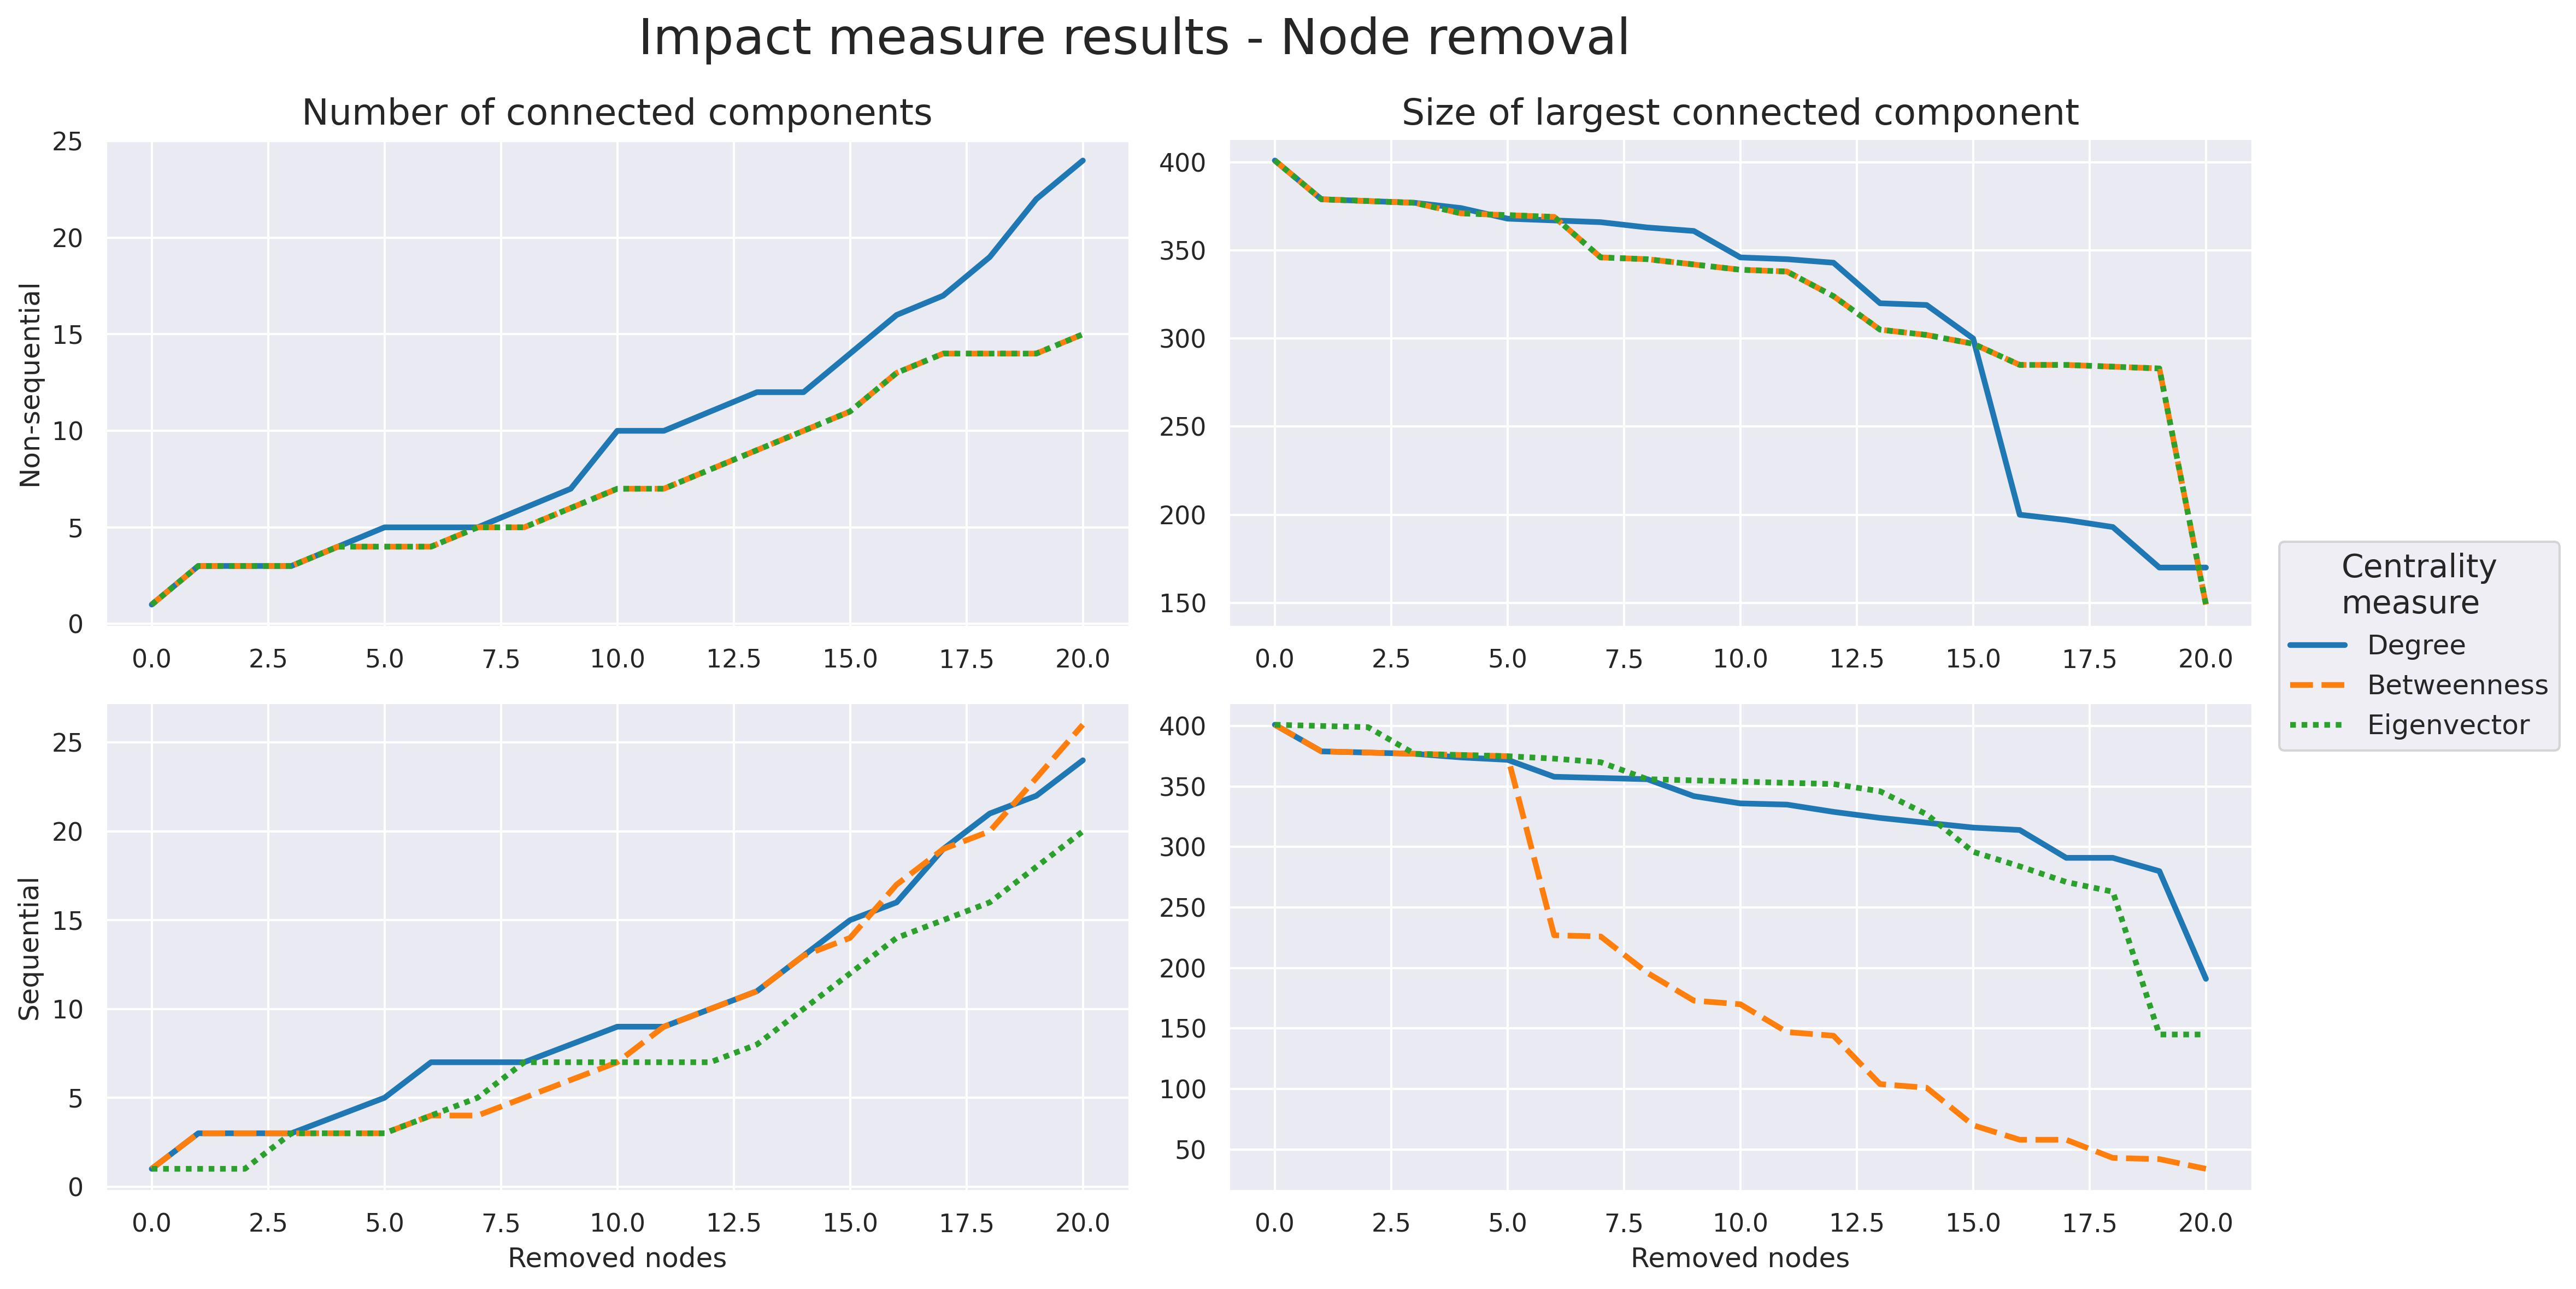
\includegraphics[width=15cm]{Results_Impact_Measures_Total.jpg}
    \caption{Result of the impact measures by non-sequential and sequential node removal strategies}
    \label{fig:impact_results}
\end{figure}

\subsection{Flows: weighted network}

\subsubsection{Adjusted centrality measures}

\subsubsection{Adjusted impact measure}

\paragraph{Total flows of the largest component}\mbox{}\\



\subsubsection{Node removal}

\section{Spatial interaction models}


\subsection{Models and calibration}

\subsubsection{Introduction}

The spatial interaction models of interest are derived from the basic gravitational model, which embodies Newton's law of universal gravitation \citep{battyUrbanModellingAlgorithms1976}. Newton's law states that a particle in the universe would interact with other particles with a force directly proportional to the product of their masses and inversely proportional to the between them \citep{battyUrbanSimulationSpatial2023}.

\paragraph{The unconstrained model}\mbox{}\\

\paragraph{Production-constrained model}\mbox{}\\

\paragraph{Attraction-constrained model}\mbox{}\\

\paragraph{Doubly constrained model}\mbox{}\\

\subsubsection{Parameter calibration}

\subsubsection{Betweenness centrality}

\subsection{Scenarios}

\subsubsection{Scenario A}

\subsubsection{Scenario B}

\subsubsection{Scenarios discussion}

% Simply use the section and subsection commands, as in this example document! With Overleaf, all the formatting and numbering is handled automatically according to the template you've chosen. If you're using Rich Text mode, you can also create new section and subsections via the buttons in the editor toolbar.

% \subsection{How to include Figures}

% First you have to upload the image file from your computer using the upload link in the file-tree menu. Then use the includegraphics command to include it in your document. Use the figure environment and the caption command to add a number and a caption to your figure. See the code for Figure \ref{fig:frog} in this section for an example.

% Note that your figure will automatically be placed in the most appropriate place for it, given the surrounding text and taking into account other figures or tables that may be close by. You can find out more about adding images to your documents in this help article on \href{https://www.overleaf.com/learn/how-to/Including_images_on_Overleaf}{including images on Overleaf}.

% \begin{figure}
% \centering
% 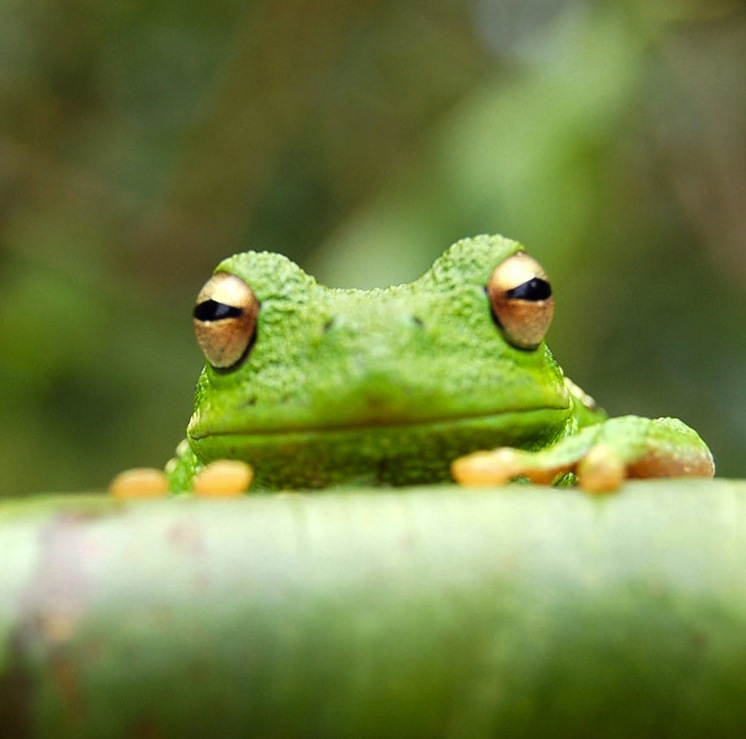
\includegraphics[width=0.3\textwidth]{frog.jpg}
% \caption{\label{fig:frog}This frog was uploaded via the file-tree menu.}
% \end{figure}

% \subsection{How to add Tables}

% Use the table and tabular environments for basic tables --- see Table~\ref{tab:widgets}, for example. For more information, please see this help article on \href{https://www.overleaf.com/learn/latex/tables}{tables}. 

% \begin{table}
% \centering
% \begin{tabular}{l|r}
% Item & Quantity \\\hline
% Widgets & 42 \\
% Gadgets & 13
% \end{tabular}
% \caption{\label{tab:widgets}An example table.}
% \end{table}

% \subsection{How to add Comments and Track Changes}

% Comments can be added to your project by highlighting some text and clicking ``Add comment'' in the top right of the editor pane. To view existing comments, click on the Review menu in the toolbar above. To reply to a comment, click on the Reply button in the lower right corner of the comment. You can close the Review pane by clicking its name on the toolbar when you're done reviewing for the time being.

% Track changes are available on all our \href{https://www.overleaf.com/user/subscription/plans}{premium plans}, and can be toggled on or off using the option at the top of the Review pane. Track changes allow you to keep track of every change made to the document, along with the person making the change. 

% \subsection{How to add Lists}

% You can make lists with automatic numbering \dots

% \begin{enumerate}
% \item Like this,
% \item and like this.
% \end{enumerate}
% \dots or bullet points \dots
% \begin{itemize}
% \item Like this,
% \item and like this.
% \end{itemize}

% \subsection{How to write Mathematics}

% \LaTeX{} is great at typesetting mathematics. Let $X_1, X_2, \ldots, X_n$ be a sequence of independent and identically distributed random variables with $\text{E}[X_i] = \mu$ and $\text{Var}[X_i] = \sigma^2 < \infty$, and let
% \[S_n = \frac{X_1 + X_2 + \cdots + X_n}{n}
%       = \frac{1}{n}\sum_{i}^{n} X_i\]
% denote their mean. Then as $n$ approaches infinity, the random variables $\sqrt{n}(S_n - \mu)$ converge in distribution to a normal $\mathcal{N}(0, \sigma^2)$.


% \subsection{How to change the margins and paper size}

% Usually the template you're using will have the page margins and paper size set correctly for that use-case. For example, if you're using a journal article template provided by the journal publisher, that template will be formatted according to their requirements. In these cases, it's best not to alter the margins directly.

% If however you're using a more general template, such as this one, and would like to alter the margins, a common way to do so is via the geometry package. You can find the geometry package loaded in the preamble at the top of this example file, and if you'd like to learn more about how to adjust the settings, please visit this help article on \href{https://www.overleaf.com/learn/latex/page_size_and_margins}{page size and margins}.

% \subsection{How to change the document language and spell check settings}

% Overleaf supports many different languages, including multiple different languages within one document. 

% To configure the document language, simply edit the option provided to the babel package in the preamble at the top of this example project. To learn more about the different options, please visit this help article on \href{https://www.overleaf.com/learn/latex/International_language_support}{international language support}.

% To change the spell check language, simply open the Overleaf menu at the top left of the editor window, scroll down to the spell check setting, and adjust accordingly.

% \subsection{How to add Citations and a References List}

% You can simply upload a \verb|.bib| file containing your BibTeX entries, created with a tool such as JabRef. You can then cite entries from it, like this: \cite{arcaute_networks_2023}. Just remember to specify a bibliography style, as well as the filename of the \verb|.bib|. You can find a \href{https://www.overleaf.com/help/97-how-to-include-a-bibliography-using-bibtex}{video tutorial here} to learn more about BibTeX.

% If you have an \href{https://www.overleaf.com/user/subscription/plans}{upgraded account}, you can also import your Mendeley or Zotero library directly as a \verb|.bib| file, via the upload menu in the file-tree.

% \subsection{Good luck!}

% We hope you find Overleaf useful, and do take a look at our \href{https://www.overleaf.com/learn}{help library} for more tutorials and user guides! Please also let us know if you have any feedback using the Contact Us link at the bottom of the Overleaf menu --- or use the contact form at \url{https://www.overleaf.com/contact}.

% \bibliographystyle{abbrvnat}
% \setcitestyle{authoryear,open={(},close={)}}
\bibliography{my_bio}

\end{document}